% Options for packages loaded elsewhere
\PassOptionsToPackage{unicode}{hyperref}
\PassOptionsToPackage{hyphens}{url}
\PassOptionsToPackage{dvipsnames,svgnames,x11names}{xcolor}
%
\documentclass[
  letterpaper,
  DIV=11,
  numbers=noendperiod]{scrreprt}

\usepackage{amsmath,amssymb}
\usepackage{iftex}
\ifPDFTeX
  \usepackage[T1]{fontenc}
  \usepackage[utf8]{inputenc}
  \usepackage{textcomp} % provide euro and other symbols
\else % if luatex or xetex
  \usepackage{unicode-math}
  \defaultfontfeatures{Scale=MatchLowercase}
  \defaultfontfeatures[\rmfamily]{Ligatures=TeX,Scale=1}
\fi
\usepackage{lmodern}
\ifPDFTeX\else  
    % xetex/luatex font selection
\fi
% Use upquote if available, for straight quotes in verbatim environments
\IfFileExists{upquote.sty}{\usepackage{upquote}}{}
\IfFileExists{microtype.sty}{% use microtype if available
  \usepackage[]{microtype}
  \UseMicrotypeSet[protrusion]{basicmath} % disable protrusion for tt fonts
}{}
\makeatletter
\@ifundefined{KOMAClassName}{% if non-KOMA class
  \IfFileExists{parskip.sty}{%
    \usepackage{parskip}
  }{% else
    \setlength{\parindent}{0pt}
    \setlength{\parskip}{6pt plus 2pt minus 1pt}}
}{% if KOMA class
  \KOMAoptions{parskip=half}}
\makeatother
\usepackage{xcolor}
\usepackage{svg}
\setlength{\emergencystretch}{3em} % prevent overfull lines
\setcounter{secnumdepth}{5}
% Make \paragraph and \subparagraph free-standing
\ifx\paragraph\undefined\else
  \let\oldparagraph\paragraph
  \renewcommand{\paragraph}[1]{\oldparagraph{#1}\mbox{}}
\fi
\ifx\subparagraph\undefined\else
  \let\oldsubparagraph\subparagraph
  \renewcommand{\subparagraph}[1]{\oldsubparagraph{#1}\mbox{}}
\fi

\usepackage{color}
\usepackage{fancyvrb}
\newcommand{\VerbBar}{|}
\newcommand{\VERB}{\Verb[commandchars=\\\{\}]}
\DefineVerbatimEnvironment{Highlighting}{Verbatim}{commandchars=\\\{\}}
% Add ',fontsize=\small' for more characters per line
\usepackage{framed}
\definecolor{shadecolor}{RGB}{241,243,245}
\newenvironment{Shaded}{\begin{snugshade}}{\end{snugshade}}
\newcommand{\AlertTok}[1]{\textcolor[rgb]{0.68,0.00,0.00}{#1}}
\newcommand{\AnnotationTok}[1]{\textcolor[rgb]{0.37,0.37,0.37}{#1}}
\newcommand{\AttributeTok}[1]{\textcolor[rgb]{0.40,0.45,0.13}{#1}}
\newcommand{\BaseNTok}[1]{\textcolor[rgb]{0.68,0.00,0.00}{#1}}
\newcommand{\BuiltInTok}[1]{\textcolor[rgb]{0.00,0.23,0.31}{#1}}
\newcommand{\CharTok}[1]{\textcolor[rgb]{0.13,0.47,0.30}{#1}}
\newcommand{\CommentTok}[1]{\textcolor[rgb]{0.37,0.37,0.37}{#1}}
\newcommand{\CommentVarTok}[1]{\textcolor[rgb]{0.37,0.37,0.37}{\textit{#1}}}
\newcommand{\ConstantTok}[1]{\textcolor[rgb]{0.56,0.35,0.01}{#1}}
\newcommand{\ControlFlowTok}[1]{\textcolor[rgb]{0.00,0.23,0.31}{#1}}
\newcommand{\DataTypeTok}[1]{\textcolor[rgb]{0.68,0.00,0.00}{#1}}
\newcommand{\DecValTok}[1]{\textcolor[rgb]{0.68,0.00,0.00}{#1}}
\newcommand{\DocumentationTok}[1]{\textcolor[rgb]{0.37,0.37,0.37}{\textit{#1}}}
\newcommand{\ErrorTok}[1]{\textcolor[rgb]{0.68,0.00,0.00}{#1}}
\newcommand{\ExtensionTok}[1]{\textcolor[rgb]{0.00,0.23,0.31}{#1}}
\newcommand{\FloatTok}[1]{\textcolor[rgb]{0.68,0.00,0.00}{#1}}
\newcommand{\FunctionTok}[1]{\textcolor[rgb]{0.28,0.35,0.67}{#1}}
\newcommand{\ImportTok}[1]{\textcolor[rgb]{0.00,0.46,0.62}{#1}}
\newcommand{\InformationTok}[1]{\textcolor[rgb]{0.37,0.37,0.37}{#1}}
\newcommand{\KeywordTok}[1]{\textcolor[rgb]{0.00,0.23,0.31}{#1}}
\newcommand{\NormalTok}[1]{\textcolor[rgb]{0.00,0.23,0.31}{#1}}
\newcommand{\OperatorTok}[1]{\textcolor[rgb]{0.37,0.37,0.37}{#1}}
\newcommand{\OtherTok}[1]{\textcolor[rgb]{0.00,0.23,0.31}{#1}}
\newcommand{\PreprocessorTok}[1]{\textcolor[rgb]{0.68,0.00,0.00}{#1}}
\newcommand{\RegionMarkerTok}[1]{\textcolor[rgb]{0.00,0.23,0.31}{#1}}
\newcommand{\SpecialCharTok}[1]{\textcolor[rgb]{0.37,0.37,0.37}{#1}}
\newcommand{\SpecialStringTok}[1]{\textcolor[rgb]{0.13,0.47,0.30}{#1}}
\newcommand{\StringTok}[1]{\textcolor[rgb]{0.13,0.47,0.30}{#1}}
\newcommand{\VariableTok}[1]{\textcolor[rgb]{0.07,0.07,0.07}{#1}}
\newcommand{\VerbatimStringTok}[1]{\textcolor[rgb]{0.13,0.47,0.30}{#1}}
\newcommand{\WarningTok}[1]{\textcolor[rgb]{0.37,0.37,0.37}{\textit{#1}}}

\providecommand{\tightlist}{%
  \setlength{\itemsep}{0pt}\setlength{\parskip}{0pt}}\usepackage{longtable,booktabs,array}
\usepackage{calc} % for calculating minipage widths
% Correct order of tables after \paragraph or \subparagraph
\usepackage{etoolbox}
\makeatletter
\patchcmd\longtable{\par}{\if@noskipsec\mbox{}\fi\par}{}{}
\makeatother
% Allow footnotes in longtable head/foot
\IfFileExists{footnotehyper.sty}{\usepackage{footnotehyper}}{\usepackage{footnote}}
\makesavenoteenv{longtable}
\usepackage{graphicx}
\makeatletter
\def\maxwidth{\ifdim\Gin@nat@width>\linewidth\linewidth\else\Gin@nat@width\fi}
\def\maxheight{\ifdim\Gin@nat@height>\textheight\textheight\else\Gin@nat@height\fi}
\makeatother
% Scale images if necessary, so that they will not overflow the page
% margins by default, and it is still possible to overwrite the defaults
% using explicit options in \includegraphics[width, height, ...]{}
\setkeys{Gin}{width=\maxwidth,height=\maxheight,keepaspectratio}
% Set default figure placement to htbp
\makeatletter
\def\fps@figure{htbp}
\makeatother
\newlength{\cslhangindent}
\setlength{\cslhangindent}{1.5em}
\newlength{\csllabelwidth}
\setlength{\csllabelwidth}{3em}
\newlength{\cslentryspacingunit} % times entry-spacing
\setlength{\cslentryspacingunit}{\parskip}
\newenvironment{CSLReferences}[2] % #1 hanging-ident, #2 entry spacing
 {% don't indent paragraphs
  \setlength{\parindent}{0pt}
  % turn on hanging indent if param 1 is 1
  \ifodd #1
  \let\oldpar\par
  \def\par{\hangindent=\cslhangindent\oldpar}
  \fi
  % set entry spacing
  \setlength{\parskip}{#2\cslentryspacingunit}
 }%
 {}
\usepackage{calc}
\newcommand{\CSLBlock}[1]{#1\hfill\break}
\newcommand{\CSLLeftMargin}[1]{\parbox[t]{\csllabelwidth}{#1}}
\newcommand{\CSLRightInline}[1]{\parbox[t]{\linewidth - \csllabelwidth}{#1}\break}
\newcommand{\CSLIndent}[1]{\hspace{\cslhangindent}#1}

\KOMAoption{captions}{tableheading}
\makeatletter
\@ifpackageloaded{tcolorbox}{}{\usepackage[skins,breakable]{tcolorbox}}
\@ifpackageloaded{fontawesome5}{}{\usepackage{fontawesome5}}
\definecolor{quarto-callout-color}{HTML}{909090}
\definecolor{quarto-callout-note-color}{HTML}{0758E5}
\definecolor{quarto-callout-important-color}{HTML}{CC1914}
\definecolor{quarto-callout-warning-color}{HTML}{EB9113}
\definecolor{quarto-callout-tip-color}{HTML}{00A047}
\definecolor{quarto-callout-caution-color}{HTML}{FC5300}
\definecolor{quarto-callout-color-frame}{HTML}{acacac}
\definecolor{quarto-callout-note-color-frame}{HTML}{4582ec}
\definecolor{quarto-callout-important-color-frame}{HTML}{d9534f}
\definecolor{quarto-callout-warning-color-frame}{HTML}{f0ad4e}
\definecolor{quarto-callout-tip-color-frame}{HTML}{02b875}
\definecolor{quarto-callout-caution-color-frame}{HTML}{fd7e14}
\makeatother
\makeatletter
\makeatother
\makeatletter
\@ifpackageloaded{bookmark}{}{\usepackage{bookmark}}
\makeatother
\makeatletter
\@ifpackageloaded{caption}{}{\usepackage{caption}}
\AtBeginDocument{%
\ifdefined\contentsname
  \renewcommand*\contentsname{Table of contents}
\else
  \newcommand\contentsname{Table of contents}
\fi
\ifdefined\listfigurename
  \renewcommand*\listfigurename{List of Figures}
\else
  \newcommand\listfigurename{List of Figures}
\fi
\ifdefined\listtablename
  \renewcommand*\listtablename{List of Tables}
\else
  \newcommand\listtablename{List of Tables}
\fi
\ifdefined\figurename
  \renewcommand*\figurename{Figure}
\else
  \newcommand\figurename{Figure}
\fi
\ifdefined\tablename
  \renewcommand*\tablename{Table}
\else
  \newcommand\tablename{Table}
\fi
}
\@ifpackageloaded{float}{}{\usepackage{float}}
\floatstyle{ruled}
\@ifundefined{c@chapter}{\newfloat{codelisting}{h}{lop}}{\newfloat{codelisting}{h}{lop}[chapter]}
\floatname{codelisting}{Listing}
\newcommand*\listoflistings{\listof{codelisting}{List of Listings}}
\makeatother
\makeatletter
\@ifpackageloaded{caption}{}{\usepackage{caption}}
\@ifpackageloaded{subcaption}{}{\usepackage{subcaption}}
\makeatother
\makeatletter
\@ifpackageloaded{tcolorbox}{}{\usepackage[skins,breakable]{tcolorbox}}
\makeatother
\makeatletter
\@ifundefined{shadecolor}{\definecolor{shadecolor}{rgb}{.97, .97, .97}}
\makeatother
\makeatletter
\makeatother
\makeatletter
\makeatother
\ifLuaTeX
  \usepackage{selnolig}  % disable illegal ligatures
\fi
\IfFileExists{bookmark.sty}{\usepackage{bookmark}}{\usepackage{hyperref}}
\IfFileExists{xurl.sty}{\usepackage{xurl}}{} % add URL line breaks if available
\urlstyle{same} % disable monospaced font for URLs
\hypersetup{
  pdftitle={Computational Analysis for Bioscientists},
  pdfauthor={Emma Rand},
  colorlinks=true,
  linkcolor={blue},
  filecolor={Maroon},
  citecolor={Blue},
  urlcolor={Blue},
  pdfcreator={LaTeX via pandoc}}

\title{Computational Analysis for Bioscientists}
\usepackage{etoolbox}
\makeatletter
\providecommand{\subtitle}[1]{% add subtitle to \maketitle
  \apptocmd{\@title}{\par {\large #1 \par}}{}{}
}
\makeatother
\subtitle{Data Analysis in R and what they forgot to teach you about
computers!}
\author{Emma Rand}
\date{2023-03-01}

\begin{document}
\maketitle
\ifdefined\Shaded\renewenvironment{Shaded}{\begin{tcolorbox}[boxrule=0pt, sharp corners, borderline west={3pt}{0pt}{shadecolor}, breakable, interior hidden, enhanced, frame hidden]}{\end{tcolorbox}}\fi

\renewcommand*\contentsname{Table of contents}
{
\hypersetup{linkcolor=}
\setcounter{tocdepth}{2}
\tableofcontents
}
\bookmarksetup{startatroot}

\hypertarget{welcome}{%
\chapter*{Welcome!}\label{welcome}}
\addcontentsline{toc}{chapter}{Welcome!}

\markboth{Welcome!}{Welcome!}

front page stuff

\bookmarksetup{startatroot}

\hypertarget{about-this-book}{%
\chapter{About this book}\label{about-this-book}}

:::: status ::: callout-important You are reading a work in progress.
This page is a dumping ground for ideas and not really readable. :::
::::

Who is this book for

bioscience

undergrads

It is in sections

part 1 what they forgot to teach you

focus on what causes problems for people learning to code.

part 2 Getting started with data. give summary

part 3 Data Analysis, improve name, give summary (babs 2)

When you see.. Try to answer before looking at the code

Your turn! Assign the value of \texttt{4} to a variable called
\texttt{y}:

\begin{Shaded}
\begin{Highlighting}[]
\NormalTok{y }\OtherTok{\textless{}{-}} \DecValTok{4}
\end{Highlighting}
\end{Shaded}

conventions used in this book

\part{What they forgot to teach you about computers}

\begin{tcolorbox}[enhanced jigsaw, opacitybacktitle=0.6, toprule=.15mm, arc=.35mm, colback=white, colframe=quarto-callout-important-color-frame, opacityback=0, titlerule=0mm, colbacktitle=quarto-callout-important-color!10!white, leftrule=.75mm, breakable, bottomtitle=1mm, toptitle=1mm, title=\textcolor{quarto-callout-important-color}{\faExclamation}\hspace{0.5em}{Important}, rightrule=.15mm, bottomrule=.15mm, coltitle=black, left=2mm]

You are reading a work in progress. This page is a dumping ground for
ideas and not really readable. :::

\end{tcolorbox}

Why this part

give a summary of contents

\hypertarget{operating-systems}{%
\chapter{Operating Systems}\label{operating-systems}}

:::: status ::: callout-important You are reading a work in progress.
This page is a dumping ground for ideas and not really readable. :::

\hypertarget{what-is-an-operating-system}{%
\section{what is an operating
system}\label{what-is-an-operating-system}}

\hypertarget{types-of-operating-system}{%
\section{types of operating system}\label{types-of-operating-system}}

include windows, mac, unix, tablets, android, apple

\hypertarget{differences-in-how-you-use-them}{%
\section{differences in how you use
them}\label{differences-in-how-you-use-them}}

keyboard keys and characters

For RStudio, the section on
\protect\hyperlink{keyboard-short-cuts-and-other-tips}{Keyboard
Shortcuts and tips} willhelp.

\begin{itemize}
\tightlist
\item
  enter / return
\item
  control / command
\item
  alt / option
\end{itemize}

Finder and Explorer

installing software

\hypertarget{understanding-file-systems}{%
\chapter{Understanding file systems}\label{understanding-file-systems}}

\begin{tcolorbox}[enhanced jigsaw, opacitybacktitle=0.6, toprule=.15mm, arc=.35mm, colback=white, colframe=quarto-callout-important-color-frame, opacityback=0, titlerule=0mm, colbacktitle=quarto-callout-important-color!10!white, leftrule=.75mm, breakable, bottomtitle=1mm, toptitle=1mm, title=\textcolor{quarto-callout-important-color}{\faExclamation}\hspace{0.5em}{Important}, rightrule=.15mm, bottomrule=.15mm, coltitle=black, left=2mm]

You are reading a work in progress. This page is a dumping ground for
ideas and not really readable. :::

\end{tcolorbox}

A file is a unit of storage on a computer with a name that uniquely
identifies it. Files can be of different types depending on the sort of
information held in them. The file name very often consists of two
parts, separated by a dot:

\begin{itemize}
\item
  name - the base name of the file
\item
  extension that should indicate the format or content of the file.
\end{itemize}

Some examples are report.doc, analysis.R, culture.csv and readme.txt.
The relationship between the file extension and the file type

One of the simplest types of file is a ``text file'' which contains text
characters without formatting such as bold or italics and no images or
colours. Plain text files can be opened in any text editor like Windows
Notepad or Mac's TextEdit.

Data is commonly held in text files because they can be read by many
programs

files of file plain text, markup and markdown

file extensions

the relationship between file extensions and programs

A file system contains files and folders

files systems are hierarchical

\begin{figure}

{\centering 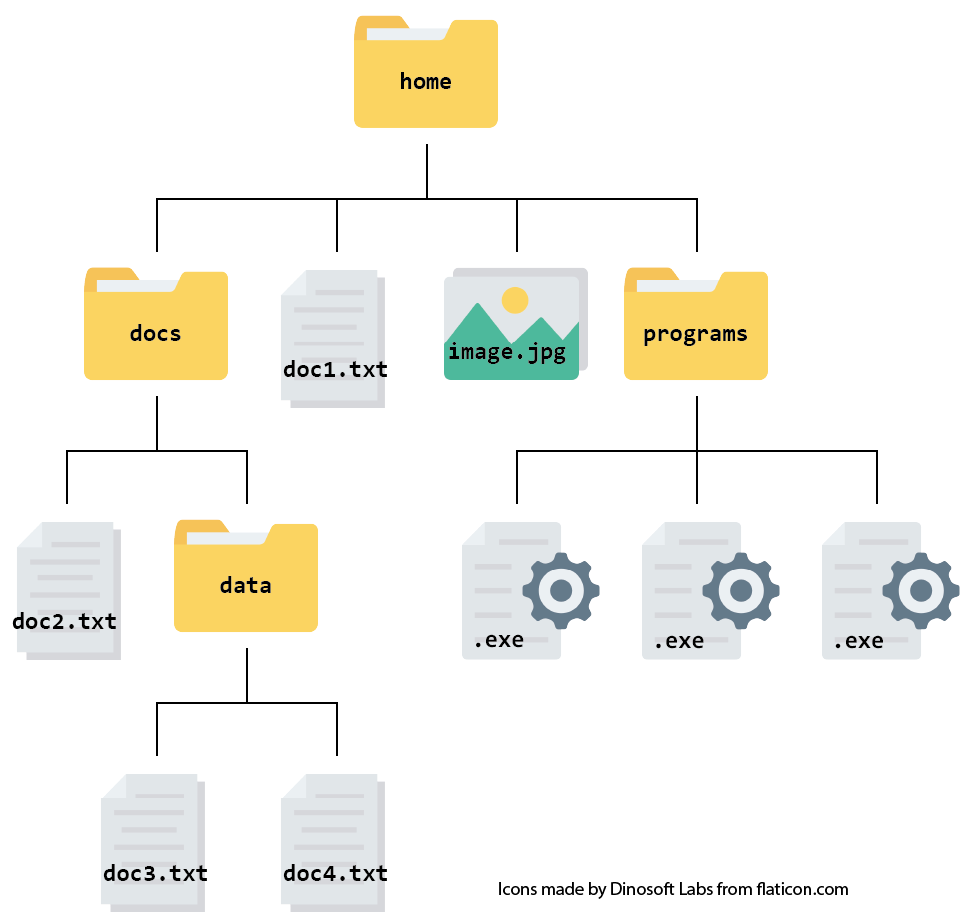
\includegraphics{images/file-system.png}

}

\caption{A file hierarchy containing 4 levels of folders and files}

\end{figure}

folder is a directory getwd(), dir() in R, cd, pwd in unix, os.getcwd()
in Python

using a file explorer, showing file extensions

Paths

root directory

typical structure on windows and mac

Working directory

Relative and absolute paths

save files fromthe internet chrome://settings/downloads

\hypertarget{organising-your-work}{%
\chapter{Organising your work}\label{organising-your-work}}

:::: status ::: callout-important You are reading a work in progress.
This page is a dumping ground for ideas and not really readable. :::

use folder

consistency

naming things

::: \{.quarto-book-part\}

\part{Getting started with data}

\begin{tcolorbox}[enhanced jigsaw, opacitybacktitle=0.6, toprule=.15mm, arc=.35mm, colback=white, colframe=quarto-callout-important-color-frame, opacityback=0, titlerule=0mm, colbacktitle=quarto-callout-important-color!10!white, leftrule=.75mm, breakable, bottomtitle=1mm, toptitle=1mm, title=\textcolor{quarto-callout-important-color}{\faExclamation}\hspace{0.5em}{Important}, rightrule=.15mm, bottomrule=.15mm, coltitle=black, left=2mm]

You are reading a work in progress. This page is a dumping ground for
ideas and not really readable. :::

\end{tcolorbox}

why this part

summary of the chapters

general ideas about data and data types

first steps with rstudio

working with data in RStudio

\hypertarget{ideas-about-data}{%
\chapter{Ideas about data}\label{ideas-about-data}}

\begin{tcolorbox}[enhanced jigsaw, opacitybacktitle=0.6, toprule=.15mm, arc=.35mm, colback=white, colframe=quarto-callout-important-color-frame, opacityback=0, titlerule=0mm, colbacktitle=quarto-callout-important-color!10!white, leftrule=.75mm, breakable, bottomtitle=1mm, toptitle=1mm, title=\textcolor{quarto-callout-important-color}{\faExclamation}\hspace{0.5em}{Important}, rightrule=.15mm, bottomrule=.15mm, coltitle=black, left=2mm]

You are reading a work in progress. This page is a dumping ground for
ideas and not really readable. :::

\end{tcolorbox}

This chapter covers some important concepts data. Data is made up of
properties we have measured or recorded, known as variables, and
observations, the individual things with those properties. Data is most
commonly (and helpfully) organised with variables in columns and each
observation on a row.

We can define a variable in two main ways:

\begin{enumerate}
\def\labelenumi{\arabic{enumi}.}
\tightlist
\item
  by what kinds of value it can take and how frequently each of its
  possible values occur
\item
  by what role the variable takes in analysis
\end{enumerate}

Both of these determine how we summarise, plot and analyse data.

\hypertarget{role-in-analysis}{%
\section{Role in analysis}\label{role-in-analysis}}

When we do research, we typically have variables that we choose or set
and variables that we measure. The variables we choose or set are called
independent or explanatory variables. The variables we measure are
called dependent or response variables.

TODO: examples

\hypertarget{kinds-of-value-data-types}{%
\section{Kinds of value: data types}\label{kinds-of-value-data-types}}

The types of values a variable can take determines how we summarise,
plot and analyse them. Sometimes this is obvious - when you can recorded
the colour of an observation you can't find the mean colour of the
sample but you can report the most common colour.

An important distinction is between discrete and continuous types of
data. Continuous variables are measurements that can take any value in
their range. Discrete variables can take only specific values.

\hypertarget{discrete-data}{%
\subsection{Discrete data}\label{discrete-data}}

Discrete variables can take only specific values, like genotype or the
number of leaves

\hypertarget{nominal-and-ordinal}{%
\subsubsection{Nominal and Ordinal}\label{nominal-and-ordinal}}

Nominal and ordinal data are categorical and often act as explanatory
variables.\\
Nominal variable have no particular order, for example, the eye colour
of Drosophila or the genotype of a mouse. When summarising data on eye
colour, it wouldn't matter what order the information was given or
plotted. Ordinal variables have an order. The Likert scale used in
questionnaires is one example. The possible responses are Strongly
agree, Agree, Disagree and Strongly disagree; these have an order that
you would use when plotting them.

Summarising nominal or ordinal data The most appropriate way to
summarise nominal or ordinal data is to report the most frequent values
or tabulate the number of each value.

\hypertarget{counts}{%
\subsubsection{Counts}\label{counts}}

Counts are one of the most common data types. They are quantitative but
discrete because they can take only specific values

\hypertarget{continuous-data}{%
\subsection{Continuous data}\label{continuous-data}}

Continuous variables are measurements that can take \emph{any} value in
their range so there are an infinite number of possible values. The
values have decimal places. Variables like the length and mass of an
organism, the volume and optical density of a solution, or the colour
intensity of an image are continuous. Many response variables are
continuous but continuous variables can also be explanatory. For
example,

\hypertarget{distributions}{%
\section{Distributions}\label{distributions}}

The distribution of a variable describes the types of values it can take
and the likelihood of each value occurring. For example, for a variable
like human height values of 1.65 metres occur more often than values of
2 metres and values of 3 metres never occur.

\begin{Shaded}
\begin{Highlighting}[]
\NormalTok{m }\OtherTok{\textless{}{-}} \FloatTok{1.65}
\NormalTok{sd }\OtherTok{\textless{}{-}} \FloatTok{0.06}
\FunctionTok{ggplot}\NormalTok{(}\AttributeTok{data =} \FunctionTok{data.frame}\NormalTok{(}\AttributeTok{Height =} \FunctionTok{c}\NormalTok{(m }\SpecialCharTok{{-}} \DecValTok{3} \SpecialCharTok{*}\NormalTok{ sd, m }\SpecialCharTok{+} \DecValTok{3} \SpecialCharTok{*}\NormalTok{ sd)), }\FunctionTok{aes}\NormalTok{(Height)) }\SpecialCharTok{+}
  \FunctionTok{stat\_function}\NormalTok{(}\AttributeTok{fun =}\NormalTok{ dnorm, }\AttributeTok{n =} \DecValTok{101}\NormalTok{, }
                \AttributeTok{args =} \FunctionTok{list}\NormalTok{(}\AttributeTok{mean =}\NormalTok{ m, }\AttributeTok{sd =}\NormalTok{ sd)) }\SpecialCharTok{+}
  \FunctionTok{scale\_y\_continuous}\NormalTok{(}\AttributeTok{breaks =} \ConstantTok{NULL}\NormalTok{, }\AttributeTok{name =} \StringTok{""}\NormalTok{,}
                     \AttributeTok{expand =} \FunctionTok{c}\NormalTok{(}\DecValTok{0}\NormalTok{, }\DecValTok{0}\NormalTok{)) }\SpecialCharTok{+}
  \FunctionTok{annotate}\NormalTok{(}\StringTok{"text"}\NormalTok{, }\AttributeTok{x =} \FloatTok{1.5}\NormalTok{, }\AttributeTok{y =} \FloatTok{4.5}\NormalTok{,}
           \AttributeTok{label =} \StringTok{"Values are rare"}\NormalTok{) }\SpecialCharTok{+}
    \FunctionTok{annotate}\NormalTok{(}\StringTok{"text"}\NormalTok{, }\AttributeTok{x =} \FloatTok{1.65}\NormalTok{, }\AttributeTok{y =} \FloatTok{4.5}\NormalTok{,}
           \AttributeTok{label =} \StringTok{"Values are common"}\NormalTok{) }\SpecialCharTok{+}
    \FunctionTok{annotate}\NormalTok{(}\StringTok{"text"}\NormalTok{, }\AttributeTok{x =} \FloatTok{1.8}\NormalTok{, }\AttributeTok{y =} \FloatTok{4.5}\NormalTok{,}
           \AttributeTok{label =} \StringTok{"Values are rare"}\NormalTok{) }\SpecialCharTok{+}
  \FunctionTok{theme\_classic}\NormalTok{()}
\end{Highlighting}
\end{Shaded}

\begin{figure}[H]

{\centering 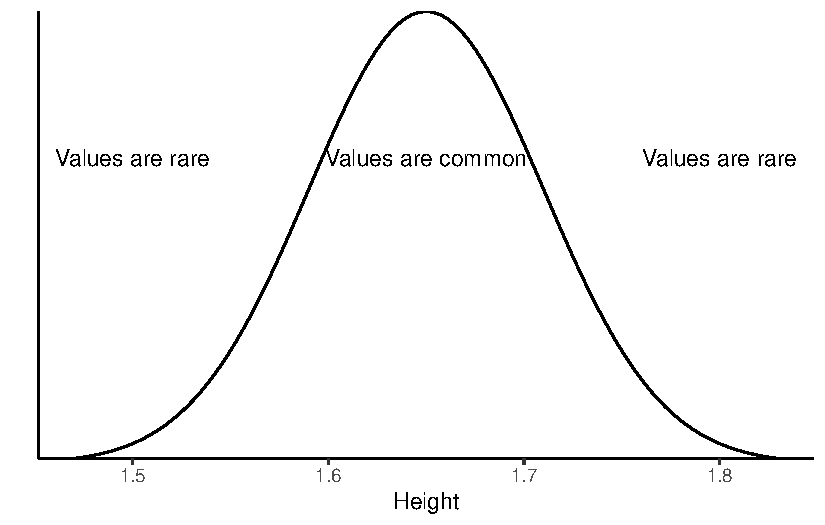
\includegraphics{ideas_about_data_files/figure-pdf/unnamed-chunk-2-1.pdf}

}

\end{figure}

\hypertarget{the-normal-distribution}{%
\subsection{The normal distribution}\label{the-normal-distribution}}

\hypertarget{distribution-of-counts}{%
\subsection{Distribution of counts}\label{distribution-of-counts}}

\hypertarget{theory-and-practice}{%
\section{Theory and practice}\label{theory-and-practice}}

The distinction between continuous and discrete values is clear in
theory but in practice, the actual values you have might differ from
what we would expect for a particular variable. For example, we would
expect the mass of cats to be continuous but if our scales only measure
to the nearest kilogram then

\begin{Shaded}
\begin{Highlighting}[]
\NormalTok{m }\OtherTok{\textless{}{-}} \DecValTok{4}
\NormalTok{sd }\OtherTok{\textless{}{-}} \FloatTok{0.8}
\FunctionTok{set.seed}\NormalTok{(}\DecValTok{1234}\NormalTok{)}
\NormalTok{a }\OtherTok{\textless{}{-}} \FunctionTok{ggplot}\NormalTok{(}\AttributeTok{data =} \FunctionTok{data.frame}\NormalTok{(}\AttributeTok{Mass =} \FunctionTok{c}\NormalTok{(m }\SpecialCharTok{{-}} \DecValTok{3} \SpecialCharTok{*}\NormalTok{ sd, m }\SpecialCharTok{+} \DecValTok{3} \SpecialCharTok{*}\NormalTok{ sd)), }\FunctionTok{aes}\NormalTok{(Mass)) }\SpecialCharTok{+}
  \FunctionTok{stat\_function}\NormalTok{(}\AttributeTok{fun =}\NormalTok{ dnorm, }\AttributeTok{n =} \DecValTok{101}\NormalTok{, }
                \AttributeTok{args =} \FunctionTok{list}\NormalTok{(}\AttributeTok{mean =}\NormalTok{ m, }\AttributeTok{sd =}\NormalTok{ sd)) }\SpecialCharTok{+} 
  \FunctionTok{scale\_y\_continuous}\NormalTok{(}\AttributeTok{breaks =} \ConstantTok{NULL}\NormalTok{, }\AttributeTok{name =} \StringTok{""}\NormalTok{, }
                     \AttributeTok{expand =} \FunctionTok{c}\NormalTok{(}\DecValTok{0}\NormalTok{, }\DecValTok{0}\NormalTok{)) }\SpecialCharTok{+}
  \FunctionTok{annotate}\NormalTok{(}\StringTok{"text"}\NormalTok{, }\AttributeTok{x =}\NormalTok{ m }\SpecialCharTok{{-}} \DecValTok{2} \SpecialCharTok{*}\NormalTok{ sd, }\AttributeTok{y =} \FloatTok{0.4}\NormalTok{,}
           \AttributeTok{label =} \StringTok{"Theory"}\NormalTok{) }\SpecialCharTok{+}
  \FunctionTok{theme\_classic}\NormalTok{()}

\NormalTok{b }\OtherTok{\textless{}{-}} \FunctionTok{ggplot}\NormalTok{(}\AttributeTok{data =} \FunctionTok{data.frame}\NormalTok{(}\AttributeTok{Mass =} \FunctionTok{round}\NormalTok{(}\FunctionTok{rnorm}\NormalTok{(}\DecValTok{1000}\NormalTok{, m, sd), }\DecValTok{0}\NormalTok{)), }\FunctionTok{aes}\NormalTok{(Mass)) }\SpecialCharTok{+}
  \FunctionTok{geom\_histogram}\NormalTok{(}\AttributeTok{binwidth =} \DecValTok{1}\NormalTok{, }\AttributeTok{colour =} \StringTok{"black"}\NormalTok{, }\AttributeTok{fill =} \StringTok{"white"}\NormalTok{) }\SpecialCharTok{+}
  \FunctionTok{scale\_y\_continuous}\NormalTok{(}\AttributeTok{breaks =} \ConstantTok{NULL}\NormalTok{, }\AttributeTok{name =} \StringTok{""}\NormalTok{,}
                     \AttributeTok{expand =} \FunctionTok{c}\NormalTok{(}\DecValTok{0}\NormalTok{, }\DecValTok{0}\NormalTok{)) }\SpecialCharTok{+}
  \FunctionTok{annotate}\NormalTok{(}\StringTok{"text"}\NormalTok{, }\AttributeTok{x =}\NormalTok{ m }\SpecialCharTok{{-}} \DecValTok{2} \SpecialCharTok{*}\NormalTok{ sd, }\AttributeTok{y =} \DecValTok{400}\NormalTok{,}
           \AttributeTok{label =} \StringTok{"Practice"}\NormalTok{) }\SpecialCharTok{+}
  \FunctionTok{theme\_classic}\NormalTok{()}

\NormalTok{a }\SpecialCharTok{+}\NormalTok{ b}
\end{Highlighting}
\end{Shaded}

\begin{figure}[H]

{\centering 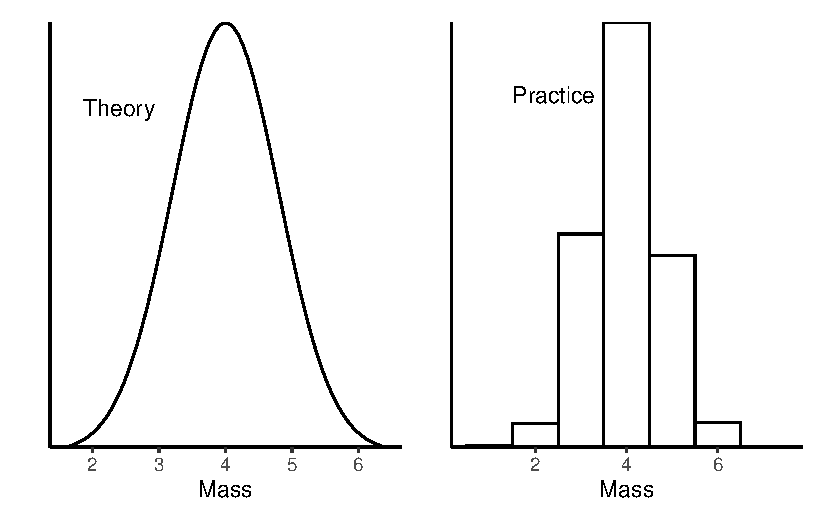
\includegraphics{ideas_about_data_files/figure-pdf/unnamed-chunk-3-1.pdf}

}

\end{figure}

\begin{Shaded}
\begin{Highlighting}[]
\NormalTok{m }\OtherTok{\textless{}{-}} \DecValTok{120000}
\NormalTok{sd }\OtherTok{\textless{}{-}} \DecValTok{20000}
\FunctionTok{set.seed}\NormalTok{(}\DecValTok{12}\NormalTok{)}
\FunctionTok{ggplot}\NormalTok{() }\SpecialCharTok{+}
  \FunctionTok{geom\_histogram}\NormalTok{(}\AttributeTok{data =} \FunctionTok{data.frame}\NormalTok{(}\AttributeTok{hairs =} \FunctionTok{round}\NormalTok{(}\FunctionTok{rnorm}\NormalTok{(}\DecValTok{60000}\NormalTok{, m, sd), }\DecValTok{0}\NormalTok{)),}
                 \FunctionTok{aes}\NormalTok{(hairs),}
                 \AttributeTok{bins =} \DecValTok{120}\NormalTok{, }\AttributeTok{colour =} \StringTok{"black"}\NormalTok{, }\AttributeTok{fill =} \StringTok{"white"}\NormalTok{) }\SpecialCharTok{+}
  \FunctionTok{scale\_y\_continuous}\NormalTok{(}\AttributeTok{breaks =} \ConstantTok{NULL}\NormalTok{, }\AttributeTok{name =} \StringTok{""}\NormalTok{,}
                     \AttributeTok{expand =} \FunctionTok{c}\NormalTok{(}\DecValTok{0}\NormalTok{, }\DecValTok{0}\NormalTok{)) }\SpecialCharTok{+}
  \FunctionTok{scale\_x\_continuous}\NormalTok{(}\StringTok{"Number of hairs on head"}\NormalTok{) }\SpecialCharTok{+}
  \FunctionTok{theme\_classic}\NormalTok{()}
\end{Highlighting}
\end{Shaded}

\begin{figure}[H]

{\centering 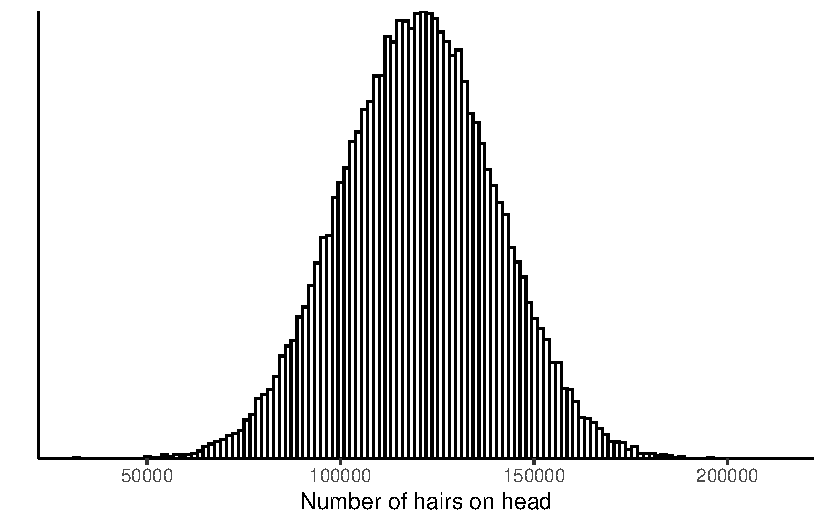
\includegraphics{ideas_about_data_files/figure-pdf/unnamed-chunk-4-1.pdf}

}

\end{figure}

\hypertarget{first-steps-in-rstudio}{%
\chapter{First Steps in RStudio}\label{first-steps-in-rstudio}}

:::: status ::: callout-important You are reading a work in progress.
This page almost readable but is a first draft and may substantial
edits. :::

This chapter starts by explaining what R and RStudio are and how you can
install them on your own machine. We introduce you to working in
RStudio, changing its appearance to suit you and to the key things you
need to know about R.

\hypertarget{what-are-r-and-rstudio}{%
\section{What are R and Rstudio?}\label{what-are-r-and-rstudio}}

\hypertarget{what-is-r}{%
\subsection{What is R?}\label{what-is-r}}

R is a programming language and environment for statistical computing
and graphics which is free and open source. It is widely used in
industry and academia. It is what is known as a ``domain-specific''
language meaning that it is designed especially for doing data analysis
and visualisation rather than a ``general-purpose'' programming language
like Python and C++. It makes doing the sorts of things that
bioscientists do a bit easier than in a general purpose-language.

\hypertarget{what-is-rstudio}{%
\subsection{What is RStudio?}\label{what-is-rstudio}}

RStudio is what is known as an ``integrated development environment''
(IDE) for R made by \href{https://posit.co/}{Posit}. IDEs have features
that make it easier to do coding like syntax highlighting, code
completion and viewers for files, code objects, packages and plots. You
don't have to use RStudio to use R but it is very helpful.

\hypertarget{why-is-it-better-to-use-r-than-excel-googlesheets-or-some-other-spreadsheet-program}{%
\subsection{Why is it better to use R than Excel, googlesheets or some
other spreadsheet
program?}\label{why-is-it-better-to-use-r-than-excel-googlesheets-or-some-other-spreadsheet-program}}

Spreadsheet programs are not statistical packages so although you can
carry out some analysis tasks in them they are
\href{https://www.gapintelligence.com/blog/understanding-r-programming-over-excel-for-data-analysis/}{limited},
get things wrong
(\href{https://www.sciencedirect.com/science/article/abs/pii/0167947394901775}{known
about since 1994}) and
\href{https://www.teampay.co/blog/biggest-excel-mistakes-of-all-time}{teach
you bad data habits}. Spreadsheets encourage you to do things that are
\href{https://datacarpentry.org/2015-05-03-NDIC/excel-ecology/02-common-mistakes.html}{going
to make analysis difficult}.

\hypertarget{why-is-it-better-to-use-r-than-spss-minitab-or-some-other-menu-driven-statistics-program}{%
\subsection{Why is it better to use R than SPSS, Minitab or some other
menu-driven statistics
program?}\label{why-is-it-better-to-use-r-than-spss-minitab-or-some-other-menu-driven-statistics-program}}

\begin{itemize}
\tightlist
\item
  R is free and open source which it will always be available to you .
\item
  Carrying out data analysis using coding makes everything you do
  reproducible
\item
  The skills and expertise you gain through learning R are highly
  transferable -- much more so than those acquired using SPSS.
\item
  See Thomas Mock's demonstration of doing some data analysis in R
  including ``The Kick Ass Curve'':
  https://rstudio.com/resources/webinars/a-gentle-introduction-to-tidy-statistics-in-r/
\end{itemize}

There are other good options such as Julia and Python and you are
encouraged to explore these. We chose R in part because of the R
community which is one of R's greatest assets, being vibrant, inclusive
and supportive of users at all levels.
https://ropensci.org/blog/2017/06/23/community/

\hypertarget{installing-r-and-rstudio}{%
\section{Installing R and Rstudio}\label{installing-r-and-rstudio}}

You will need to install both R and RStudio to use them on your own
machine. Installation is normally straightforward but you can follow a
tutorial here:
https://learnr-examples.shinyapps.io/ex-setup-r/\#section-welcome

\hypertarget{installing-r}{%
\subsection{Installing R}\label{installing-r}}

Go to \url{https://cloud.r-project.org/} and download the ``Precompiled
binary distributions of the base system and contributed packages''
appropriate for your machine.

\hypertarget{for-windows}{%
\subsubsection{For Windows}\label{for-windows}}

Click ``Download R for Windows'', then ``base'', then ``Download R
4.\#.\# for Windows''. This will download an \texttt{.exe} file. Once
downloaded, open (double click) that file to start the installation.

\hypertarget{for-mac}{%
\subsubsection{For Mac}\label{for-mac}}

Click ``Download R for (Mac) OS X'', then ``R-4.\#.\#.pkg'' to download
the installer. Run the installer to complete installation.

\hypertarget{for-linux}{%
\subsubsection{For Linux}\label{for-linux}}

Click ``Download R for Linux''. Instructions on installing are given for
Debian, Redhat, Suse and Ubuntu distributions. Where there is a choice,
install both \texttt{r-base} and \texttt{r-base-dev}.

\hypertarget{installing-r-studio}{%
\subsection{Installing R Studio}\label{installing-r-studio}}

Go to \url{https://posit.co/download/rstudio-desktop/}

\hypertarget{install-the-tidyverse-package}{%
\section{\texorpdfstring{Install the \textbf{\texttt{tidyverse}}
package}{Install the tidyverse package}}\label{install-the-tidyverse-package}}

Install \textbf{\texttt{tidyverse}}:

\begin{Shaded}
\begin{Highlighting}[]
\FunctionTok{install.packages}\NormalTok{(}\StringTok{"tidyverse"}\NormalTok{)}
\end{Highlighting}
\end{Shaded}

\hypertarget{introduction-to-rstudio}{%
\section{Introduction to RStudio}\label{introduction-to-rstudio}}

In this section we will introduce you to working in RStudio. We will
explain the windows that you see when you first open RStudio and how to
change its appearance to suit you. Then we will see how we use R as a
calculator and how assign values to R objects.

\hypertarget{changing-the-appearance}{%
\subsection{Changing the appearance}\label{changing-the-appearance}}

When you first open RStudio it will display three panes and have a white
background Figure~\ref{fig-rstudio-first-open}

\begin{figure}

{\centering 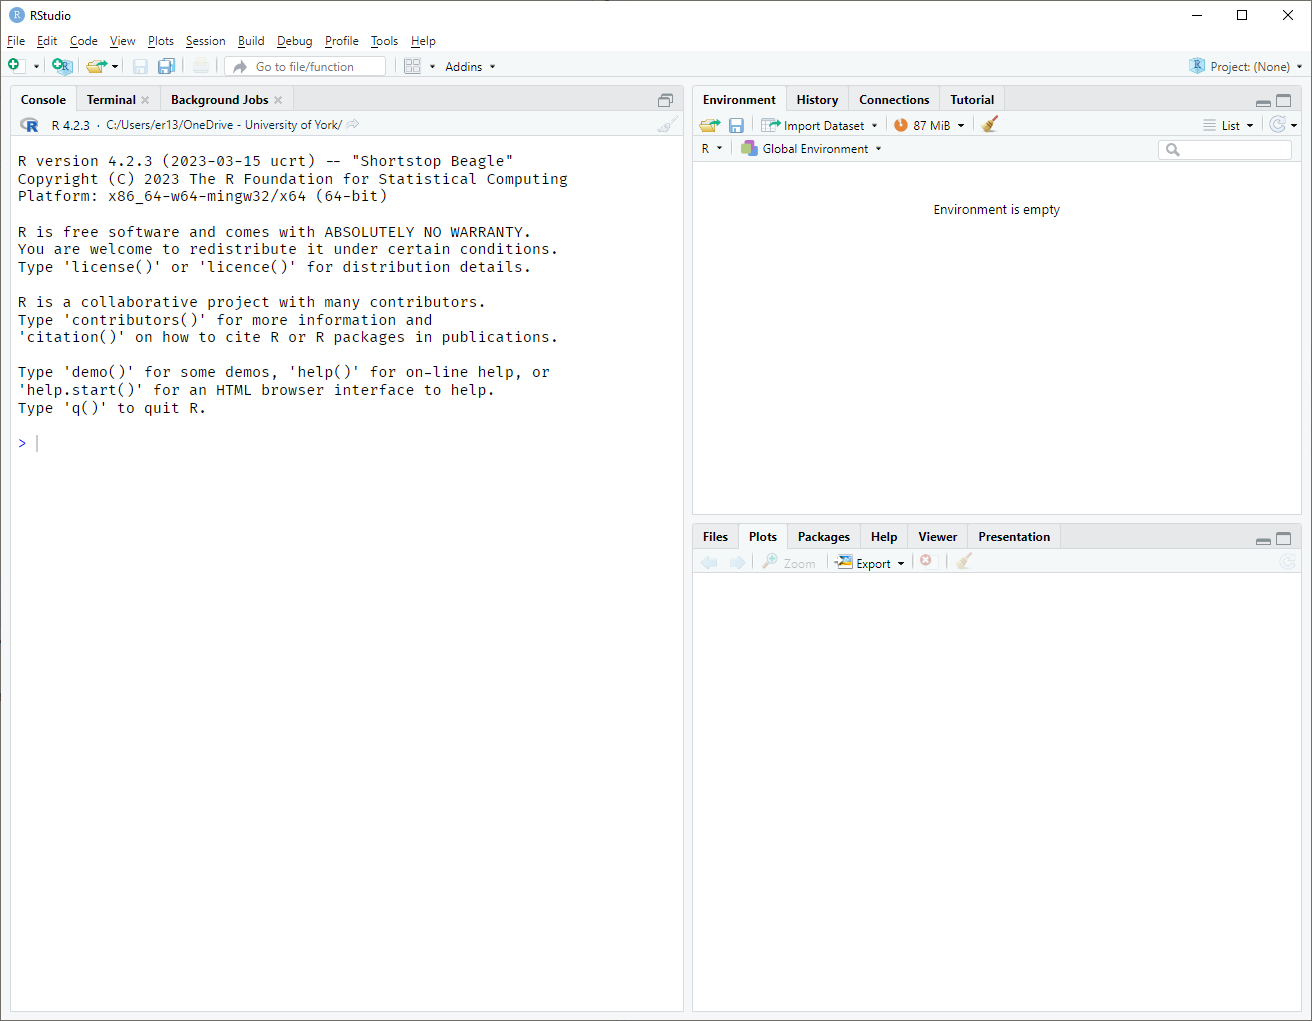
\includegraphics[width=8.33333in,height=\textheight]{images/rstudio-first-open.png}

}

\caption{\label{fig-rstudio-first-open}When you first open RStudio it
will be white with three panes}

\end{figure}

We will talk more about these three panes soon but first, let's get into
character - the character of a programmer! You might have noticed that
people comfortable around computers are often using dark backgrounds. A
dark background reduces eye strain and often makes ``code syntax'' more
obvious making it faster to learn and understand at a glance. Code
syntax is the set of rules that define what the various combinations of
symbols mean. It takes time to learn these rules and you will learn best
by repeated exposure to writing, reading and copying code. You have done
this before when you learned your first spoken language. All languages
have syntax rules governing the order of words and we rarely think about
these consciously, instead relying on what sounds and looks right. And
what sounds and looks right grows out repeated exposure. For example,
35\% of languages, including English, Chinese, Yoruba and Polish use the
Subject-Verb-Object syntax rule:

\begin{itemize}
\tightlist
\item
  English: Emma likes R
\item
  Chinese: 艾玛喜欢R Emma xǐhuān R
\item
  Yoruba: Emma fẹran R
\item
  Polish: Emma lubi R
\end{itemize}

and 40\% use Subject-Object-Verb including Turkish and Korean

\begin{itemize}
\tightlist
\item
  Turkish: Emma R'yi seviyor
\item
  Korean: 엠마는 R을 좋아한다 emmaneun Reul joh-ahanda
\end{itemize}

You learned this rule in your language very early, long before you were
conscious of it, just by being exposed to it frequently. In this book I
try to tell you the syntax rules, but you will learn most from looking
at, and copying code. Because of this, it is well worth tinkering with
the appearance of RStudio to see what Editor theme makes code elements
most obvious to you.

There is a tool bar at the top of RStudio. Choose the \texttt{Tools}
option and then \texttt{Global\ options}. This will open a window where
many options can be changed
Figure~\ref{fig-tools-global-options-appearance}.

\begin{figure}

{\centering 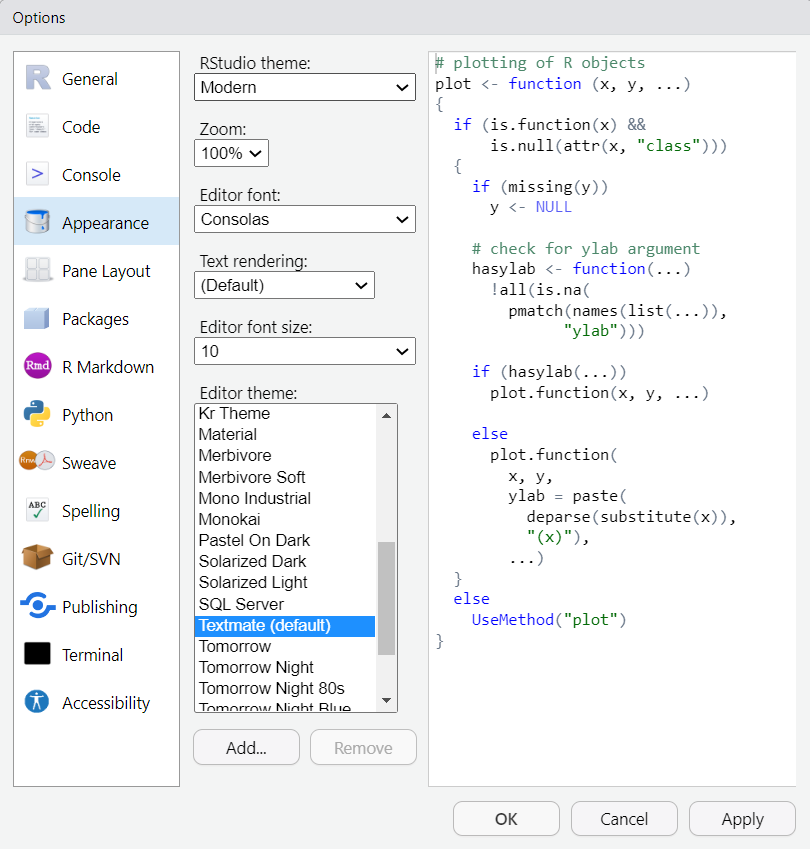
\includegraphics[width=8.33333in,height=\textheight]{images/tools-global-options-appearance.png}

}

\caption{\label{fig-tools-global-options-appearance}Tools \textbar{}
Global Options opens a window. One of the options is Appearance}

\end{figure}

Go to the \texttt{Appearance} Options and choose and Editor theme you
like, followed by OK.

The default theme is Textmate. You will notice that all the Editor
themes have syntax highlighting so that keywords, variable names,
operators, etc are coloured but some themes have stronger contrasts than
others. For beginners, I recommend Vibrant Ink, Chaos or Merbivore
rather than Dreamweaver or Gob which have little contrast between some
elements. However, individuals differ so experiment for yourself. I tend
to vary between Solarised light and dark.

You can also turn one Screen Reader Support in the Accessibility Options
in Tools \textbar{} Global Options.

Back to the Panes. You should be looking at three windows: One on the
left and two on the right\footnote{If this is not a fresh install of
  RStudio, you might be looking at fours windows, two on the left and
  two on the right. That's fine - we will al be using four shortly. For
  the time being, you might want to close the ``Script'' window using
  the small cross next to ``Untitled1''.}.

The window on the left, labelled Console, is where R commands are
executed. In a moment we will start by typing commands in this window.
Over on the right hand side, at the top, have several tabs, with the
Environment tab showing. This is where all the objects and data that you
create will be listed. Behind the Environment tab is the History and
later you will be able to view this to see a history of all your
commands.

On the bottom right hand side, we have a tab called Plots which is where
your plots will go, a tab called Files which is a file explorer just
like Windows Explorer or Mac Finder, and a Packages tab where you can
see all the packages that are installed. The Packages tab also provides
a way to install additional packages. The Help tab has access to all the
manual pages.

Right, let's start coding!

\hypertarget{your-first-piece-of-code}{%
\subsection{Your first piece of code}\label{your-first-piece-of-code}}

We can use R just like a calculator. Put your cursor after the
\texttt{\textgreater{}} in the Console, type \texttt{3\ +\ 4} and ↵
Enter to send that command:

\begin{Shaded}
\begin{Highlighting}[]
\DecValTok{3}\SpecialCharTok{+}\DecValTok{4}
\end{Highlighting}
\end{Shaded}

\begin{verbatim}
[1] 7
\end{verbatim}

The \texttt{\textgreater{}} is called the ``prompt''. You do not have to
type it, it tells you that R is ready for input.

Where I've written \texttt{3+4}, I have no spaces. However, you
\emph{can} have spaces, and in fact, it's good practice to use spaces
around your operators because it makes your code easier to read. So a
better way of writing this would be:

\begin{Shaded}
\begin{Highlighting}[]
\DecValTok{3} \SpecialCharTok{+} \DecValTok{4}
\end{Highlighting}
\end{Shaded}

\begin{verbatim}
[1] 7
\end{verbatim}

In the output we have the number \texttt{7}, which, obviously, is the
answer. From now on, you should assume commands typed at the console
should be followed by ↵ Enter to send them.

The one in parentheses, \texttt{{[}1{]}}, is an index. It is telling you
that the \texttt{7} is the first element of the output. We can see this
more clear if we create something with more output. For example,
\texttt{50:100} will print the numbers from 50 to 100.

\begin{Shaded}
\begin{Highlighting}[]
\DecValTok{50}\SpecialCharTok{:}\DecValTok{100}
\end{Highlighting}
\end{Shaded}

\begin{verbatim}
 [1]  50  51  52  53  54  55  56  57  58  59  60  61  62  63  64  65  66  67  68
[20]  69  70  71  72  73  74  75  76  77  78  79  80  81  82  83  84  85  86  87
[39]  88  89  90  91  92  93  94  95  96  97  98  99 100
\end{verbatim}

The numbers in the square parentheses at the beginning of the line give
you the index of the first element in the line. R is telling you where
you are in the output.

\hypertarget{assigning-variables}{%
\subsection{Assigning variables}\label{assigning-variables}}

Very often we want to keep input values or output for future use. We do
this with `assignment' An assignment is a statement in programming that
is used to set a value to a variable name. In R, the operator used to do
assignment is \texttt{\textless{}-}. It assigns the value on the
right-hand to the value on the left-hand side.

To assign the value \texttt{3} to \texttt{x} we do:

\begin{Shaded}
\begin{Highlighting}[]
\NormalTok{x }\OtherTok{\textless{}{-}} \DecValTok{3}
\end{Highlighting}
\end{Shaded}

and ↵ Enter to send that command.

The assignment operator is made of two characters, the
\texttt{\textless{}} and the \texttt{-} and there is a keyboard short
cut: Alt+- (windows) or Option+- (Mac). Using the shortcut means you'll
automatically get spaces. You won't see any output when the command has
been executed because there is no output. However, you will see
\texttt{x} listed under Values in the Environment tab (top right).

Your turn! Assign the value of \texttt{4} to a variable called
\texttt{y}:

\begin{Shaded}
\begin{Highlighting}[]
\NormalTok{y }\OtherTok{\textless{}{-}} \DecValTok{4}
\end{Highlighting}
\end{Shaded}

Check you can see \texttt{y} listed in the Environment tab.

Type \texttt{x} and ↵ Enter to print the contents of \texttt{x} in the
console:

\begin{Shaded}
\begin{Highlighting}[]
\NormalTok{x}
\end{Highlighting}
\end{Shaded}

\begin{verbatim}
[1] 3
\end{verbatim}

We can use these values in calculations just like we could in in maths
and algebra.

\begin{Shaded}
\begin{Highlighting}[]
\NormalTok{x }\SpecialCharTok{+}\NormalTok{ y}
\end{Highlighting}
\end{Shaded}

\begin{verbatim}
[1] 7
\end{verbatim}

We get the output of \texttt{7} just as we expect. Suppose we make a
mistake when typing, for example, accidentally pressing the u button
instead of the y button:

\begin{Shaded}
\begin{Highlighting}[]
\NormalTok{x }\SpecialCharTok{+}\NormalTok{ u}
\end{Highlighting}
\end{Shaded}

\begin{verbatim}
Error in eval(expr, envir, enclos): object 'u' not found
\end{verbatim}

We get an error. We will probably see this error quite often - it means
we have tried to use a variable that is not in our Environment. So when
you get that error, have a quick look up at your environment\footnote{When
  we are using scripts, it is very easy to write code but forget to run
  it. Very often when you see this error it will because you have
  written the code to create an object but forgotten to execute it.}.

We made a typo and will want to try again. We usefully have access to
all the commands that previously entered when we use the ↑ Up Arrow.
This is known as command recall. Pressing the ↑ Up Arrow once recalls
the last command; pressing it twice recalls the command before the last
one and so on.

Recall the \texttt{x\ +\ u} command (you may need to use the ↓ Down
Arrow to get back to get it) and use the Back space key to remove the
\texttt{u} and then add a \texttt{y}.

A lot of what we type is going to be wrong - that is not because you are
a beginner, it is same for everybody! On the whole, you type it wrong
until you get it right and then you move to the next part. This means
you are going to have to access your previous commands often. The
History - behind the Environment tab - contains everything you can see
with the ↑ Up Arrow. You can imagine that as you increase the number of
commands you run in a session, having access the this record of
everything you did is useful. However, the thing about the history is,
that it has \emph{everything} you typed, including all the wrong things!

What we really want is a record of everything we did that was right!
This is why we use scripts instead of typing directly into the console.

\hypertarget{using-scripts}{%
\subsection{Using Scripts}\label{using-scripts}}

An R script is a plain text file with a \texttt{.R} extension and
containing R code. Instead of typing into the console, we normally type
into a script and then send the commands to the console when we are
ready to run them. Then if we've made any mistakes, we just correct our
script and by the end of the session, it contains a record of everything
we typed that worked.

You have several options open a new script:

\begin{itemize}
\tightlist
\item
  button: Green circle with a white cross, top left and choose R Script
\item
  menu: File \textbar{} New File \textbar{} R Script
\item
  keyboard shortcut: Ctrl+Shift+N (Windows) / Shift+Command+N (Mac)
\end{itemize}

Open a script and add the two assignments to it:

\begin{Shaded}
\begin{Highlighting}[]
\NormalTok{x }\OtherTok{\textless{}{-}} \DecValTok{3}
\NormalTok{y }\OtherTok{\textless{}{-}} \DecValTok{4}
\end{Highlighting}
\end{Shaded}

To send the first line to the console, we place our cursor on the line
(anywhere) and press Ctrl-Enter (Windows) / Command-Return. That line
will be executed in the console and in the script, our cursor will jump
to the next line. Now, send the second command to the console in the
same way.

From this point forward, you should assume commands should be typed into
the script and sent to the console.

Add the incorrect command attempting to sum the two variables:

\begin{Shaded}
\begin{Highlighting}[]
\NormalTok{x }\SpecialCharTok{+}\NormalTok{ u}
\end{Highlighting}
\end{Shaded}

\begin{verbatim}
Error in eval(expr, envir, enclos): object 'u' not found
\end{verbatim}

To correct this, we do not add another line to the script but instead
edit the existing command:

\begin{Shaded}
\begin{Highlighting}[]
\NormalTok{x }\SpecialCharTok{+}\NormalTok{ y}
\end{Highlighting}
\end{Shaded}

\begin{verbatim}
[1] 7
\end{verbatim}

In addition to making it easy to keep a record of your work, scripts
have another big advantage, you can include `comments' - pieces of text
that describe what the code is doing. Comments are indicated with a
\texttt{\#} in front of them. You can write anything you like after a
\texttt{\#} and R will recognise that it is not code and doesn't need to
be run.

\begin{Shaded}
\begin{Highlighting}[]
\CommentTok{\# This script performs the sum of two values}

\NormalTok{x }\OtherTok{\textless{}{-}} \DecValTok{3}    \CommentTok{\# can be altered}
\NormalTok{y }\OtherTok{\textless{}{-}} \DecValTok{4}    \CommentTok{\# can be altered}

\CommentTok{\# perform sum}
\NormalTok{x }\SpecialCharTok{+}\NormalTok{ y}
\end{Highlighting}
\end{Shaded}

\begin{verbatim}
[1] 7
\end{verbatim}

The comments should be highlighted in a different colour than the code.
They will be italic in some Editor themes.

You have several options save a script:

\begin{itemize}
\tightlist
\item
  button: use the floppy disc icon
\item
  menu: File \textbar{} Save
\item
  keyboard shortcut: Ctrl+S (Windows) / Command+S (Mac)
\end{itemize}

You could use a name like \texttt{test1.R} - note the \texttt{.R}
extension wil be added automatically.

\hypertarget{other-types-of-file-in-rstudio}{%
\subsection{Other types of file in
RStudio}\label{other-types-of-file-in-rstudio}}

\begin{itemize}
\tightlist
\item
  \texttt{.R} script code but not the objects. You always want to save
  this
\item
  \texttt{.Rdata} also known as the workspace or session, the objects,
  but not the code. You usually do not want to save this. Some
  exceptions e.g., if it takes quite a long time to run the commands.
\item
  text files
\end{itemize}

I recommend changing some of the default settings to make your life a
little easier. Go back into the Global Options window with Tools
\textbar{} Global Options. The top tab is General
Figure~\ref{fig-tools-global-options-general}.

\begin{figure}

{\centering 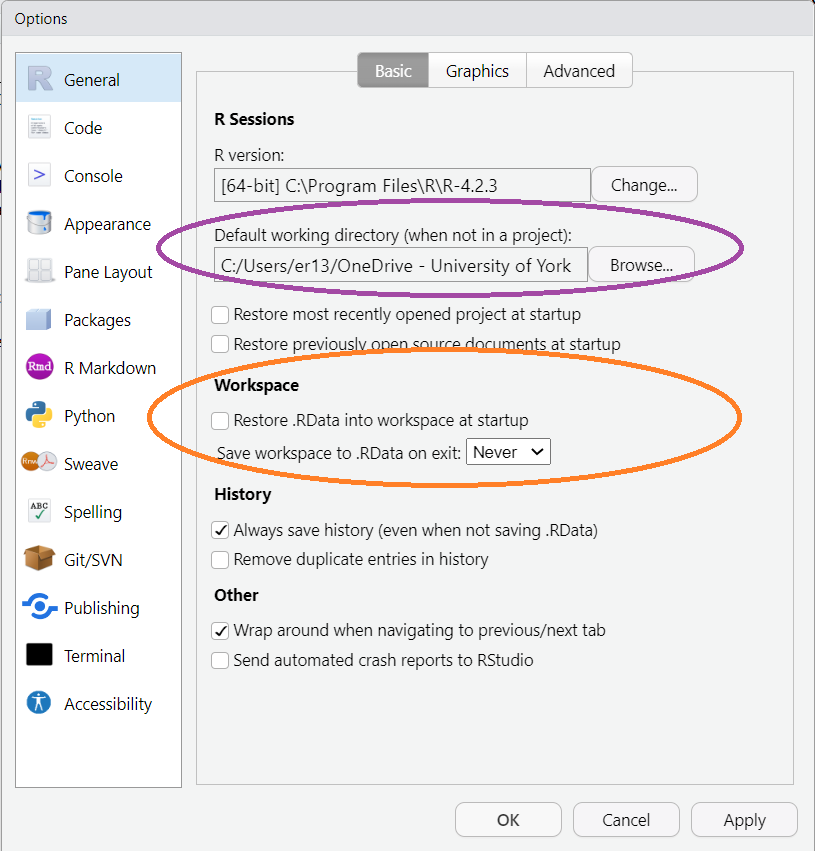
\includegraphics[width=8.33333in,height=\textheight]{images/tools-global-options-general.png}

}

\caption{\label{fig-tools-global-options-general}Tools \textbar{} Global
Options opens a window. One of the options is General. This where you
can change the default behaviour of RStudio. Highlighted is the default
(start up) directory and the option to Save and Restore the workspace.}

\end{figure}

First, we will set our default working directory. Under `Default working
directory (when not in a project\footnote{We will find out what an
  RStudio Project is very soon. You will want to use a project for most
  of your work - they make everything a little easier.}):' click Browse
and navigate to a through your file system to a folder where you want to
work. You may want to create a folder specifically for studying this
book.

Second, we will change the Workspace options. Turn off `Restore .RData
into workspace at startup' and change `Save workspace to .RData on exit'
to `Never'. These options mean R will start up clean each time.

\hypertarget{recap-of-rstudio-anatomy}{%
\section{Recap of RStudio anatomy}\label{recap-of-rstudio-anatomy}}

This figure (see Figure~\ref{fig-rstudio-anatomy}\footnote{You can zoom
  into this at the
  \href{https://www-users.york.ac.uk/~er13/RStudio\%20Anatomy.svg}{Direct
  link}}) summarises shows what each of the four RStudio panes and what
they are used for to summarise much of what we have covered so far.

\begin{figure}

{\centering \includesvg{http://www-users.york.ac.uk/~er13/RStudio\%20Anatomy.svg}

}

\caption{\label{fig-rstudio-anatomy}A screenshot of RStudio's four panes
annotated with what each pane is for.}

\end{figure}

\hypertarget{data-types-and-structures-in-r}{%
\section{Data types and structures in
R}\label{data-types-and-structures-in-r}}

In this section, we are going to introduce you to some of R's data types
and structures. We won't be covering all of them now, just those you are
going to use often in this part of the book. These are numerics
(numbers), characters, `logicals', vectors and dataframes. We can do a
lot with just these. We will also cover using functions.

We are going to consider

\begin{itemize}
\item
  types of value also known as data types
\item
  functions
\item
  data structures
\end{itemize}

\hypertarget{data-types}{%
\subsection{Data types}\label{data-types}}

This refers to the type of value that something is. They might be
numerics or characters or `logical' (either true of false). We assign a
number, like the value of 23 to a variable called \texttt{x} like this:

\begin{Shaded}
\begin{Highlighting}[]
\NormalTok{x }\OtherTok{\textless{}{-}} \DecValTok{23}
\NormalTok{x}
\end{Highlighting}
\end{Shaded}

\begin{verbatim}
[1] 23
\end{verbatim}

We do not need to use quotes for numbers but we do need to use them for
characters and can assign the word banana to the variable \texttt{a}
like this:

\begin{Shaded}
\begin{Highlighting}[]
\NormalTok{a }\OtherTok{\textless{}{-}} \StringTok{"banana"}
\NormalTok{a}
\end{Highlighting}
\end{Shaded}

\begin{verbatim}
[1] "banana"
\end{verbatim}

Quotes are needed because otherwise R wouldn't know whether you were
referring to a value or a existing object called \texttt{banana}. This
is also why you can't have variable name like \texttt{14} - R would not
be able to tell the difference between the number 14 and an object named
\texttt{14} since numbers and objects don't need quotes.

Anything composed of non-numeric characters, including single
characters, need to have quotes around it. You can even force a number
to be a character by putting quotes around it:

\begin{Shaded}
\begin{Highlighting}[]
\NormalTok{b }\OtherTok{\textless{}{-}} \StringTok{"23"}
\NormalTok{b}
\end{Highlighting}
\end{Shaded}

\begin{verbatim}
[1] "23"
\end{verbatim}

Notice that things inside quotes appear in a different colour (the
colour will depend on the Editor theme you choose). This will help you
identify when you have forgotten some closing quotes\footnote{RStudio
  makes it hard for you to forget closing quotes and parentheses because
  when you type an opening quote or parenthesis, it automatically adds
  its closing partner. When people are learning they are sometimes
  tempted to delete these so they can type what goes inside the
  quotes/parentheses and then manually add the closing partner. I
  strongly recommend you don't not delete them. RStudio adds the closing
  character but it leaves your cursor in the right position to complete
  the contents.}:

\begin{Shaded}
\begin{Highlighting}[]
\NormalTok{a }\OtherTok{\textless{}{-}} \StringTok{"banana}
\StringTok{x \textless{}{-} 23}
\end{Highlighting}
\end{Shaded}

Although the data type is `character' we often use the term `string' for
collections - strings - of characters

We also have special values called `logicals' which take a value of
either \texttt{TRUE} or \texttt{FALSE.}

\begin{Shaded}
\begin{Highlighting}[]
\NormalTok{c }\OtherTok{\textless{}{-}} \ConstantTok{TRUE}
\NormalTok{c}
\end{Highlighting}
\end{Shaded}

\begin{verbatim}
[1] TRUE
\end{verbatim}

Although \texttt{TRUE} is a word, R recognises it as special word. It
appears in a different colour and no quotes are needed. This is the same
for \texttt{FALSE}.

\begin{Shaded}
\begin{Highlighting}[]
\NormalTok{c }\OtherTok{\textless{}{-}} \ConstantTok{FALSE}
\NormalTok{c}
\end{Highlighting}
\end{Shaded}

\begin{verbatim}
[1] FALSE
\end{verbatim}

As you type \texttt{FALSE}, the colour changes as it recognises the
special word \texttt{FALSE}. Try to pay attention to the editor theme's
colouring - it is trying to help you!

\hypertarget{functions}{%
\subsection{Functions}\label{functions}}

The aim of this section is to help you understand the logic of using a
function. Functions have a name and then a set of parentheses. The
function name minimally explains what the function does. Inside the
parentheses are `arguments' - the pieces of information you give to the
function. When coding, we often talk about passing arguments to
functions and calling functions. A simple function call looks like this:

\begin{Shaded}
\begin{Highlighting}[]
\FunctionTok{function\_name}\NormalTok{(argument)}
\end{Highlighting}
\end{Shaded}

A function can take zero to many arguments. Where you give several
arguments, they are separated by commas:

\begin{Shaded}
\begin{Highlighting}[]
\FunctionTok{function\_name}\NormalTok{(argument1, argument2, argument3, ...)}
\end{Highlighting}
\end{Shaded}

The first function you are going to use is \texttt{str()} which gives
the \textbf{str}ucture of an object:

\begin{Shaded}
\begin{Highlighting}[]
\FunctionTok{str}\NormalTok{(x)}
\end{Highlighting}
\end{Shaded}

\begin{verbatim}
 num 23
\end{verbatim}

It's telling me that \texttt{x} is a number and contains 23.

Your turn! Use \texttt{str()} on \texttt{b}:

\begin{Shaded}
\begin{Highlighting}[]
\FunctionTok{str}\NormalTok{(b)}
\end{Highlighting}
\end{Shaded}

\begin{verbatim}
 chr "23"
\end{verbatim}

\texttt{str()} is a function I use a lot to check what sort of R object
I have.

We must give \texttt{str()} at least one argument, the object we want
the structure of, but additional arguments are also possible. Later we
will discover how to find out and use a function's arguments.

So far we our objects have consisted of a single thing but usually we
have several bits of data that we want to collect together into a data
structure.

\hypertarget{data-structures-vectors}{%
\subsection{Data structures: vectors}\label{data-structures-vectors}}

Imagine we have the ages of six people. Since all the numbers are ages,
we would want to keep them together. The minimal data structure is
called a vector. We can create a vector, which collects together several
numbers using a function, \texttt{c()}. This is one of only a few
functions in R with a single-letter name. Because it has a single
letter, sometimes people get confused about it but we can tell it is a
function because it has a set of parentheses.

To create a vector called \texttt{ages} of several numbers we use

\begin{Shaded}
\begin{Highlighting}[]
\NormalTok{ages }\OtherTok{\textless{}{-}} \FunctionTok{c}\NormalTok{(}\DecValTok{23}\NormalTok{, }\DecValTok{42}\NormalTok{, }\DecValTok{7}\NormalTok{, }\DecValTok{9}\NormalTok{, }\DecValTok{54}\NormalTok{, }\DecValTok{12}\NormalTok{)}
\end{Highlighting}
\end{Shaded}

Type \texttt{ages} and run if you want to print the contents to the
console:

\begin{Shaded}
\begin{Highlighting}[]
\NormalTok{ages}
\end{Highlighting}
\end{Shaded}

\begin{verbatim}
[1] 23 42  7  9 54 12
\end{verbatim}

Using \texttt{str()} on \texttt{ages}

\begin{Shaded}
\begin{Highlighting}[]
\FunctionTok{str}\NormalTok{(ages)}
\end{Highlighting}
\end{Shaded}

\begin{verbatim}
 num [1:6] 23 42 7 9 54 12
\end{verbatim}

tells us we have numbers with the indices of 1 to 6.

We can also create a vector of strings. Suppose we have names to go with
the ages.

\begin{Shaded}
\begin{Highlighting}[]
\NormalTok{names }\OtherTok{\textless{}{-}} \FunctionTok{c}\NormalTok{(}\StringTok{"Rowan"}\NormalTok{, }\StringTok{"Aang"}\NormalTok{, }\StringTok{"Zain"}\NormalTok{, }\StringTok{"Charlie"}\NormalTok{, }\StringTok{"Jules"}\NormalTok{, }\StringTok{"Efe"}\NormalTok{)}
\end{Highlighting}
\end{Shaded}

RStudio has a super useful feature for putting items in quotes, brackets
or parentheses if you initially forget them: If you select something and
type the opening element, that thing will be surrounded rather than over
written. For example, if you had written:

\begin{Shaded}
\begin{Highlighting}[]
\NormalTok{names }\OtherTok{\textless{}{-}}\NormalTok{ Rowan, Aang, Zain, Charlie, Jules, Efe}
\end{Highlighting}
\end{Shaded}

Select one of the names and then type an opening quote - you should see
the name is then surrounded by quotes rather than overwritten. You can
repeat this process for all the names (note that double clicking on the
name will select it). Selecting the whole list and typing an opening
parenthesis will put the whole list in parentheses. This is a feature
you get to love so much and use so often that other programs will annoy
you when you overwrite something you meant to quote!

So we can also have vectors of logical values. For example, we might
have a vector that indicates that Rowan, Aang and Charlie like
chocolate, but Zain, Jules and Efe do not:

\begin{Shaded}
\begin{Highlighting}[]
\NormalTok{chocolate }\OtherTok{\textless{}{-}} \FunctionTok{c}\NormalTok{(}\ConstantTok{TRUE}\NormalTok{, }\ConstantTok{TRUE}\NormalTok{, }\ConstantTok{FALSE}\NormalTok{, }\ConstantTok{TRUE}\NormalTok{, }\ConstantTok{FALSE}\NormalTok{, }\ConstantTok{FALSE}\NormalTok{)}
\end{Highlighting}
\end{Shaded}

Remember, because \texttt{TRUE} and \texttt{FALSE} are special words so
we do not need quote them.

\hypertarget{indexing-vectors}{%
\subsection{Indexing vectors}\label{indexing-vectors}}

You might be wondering how to get a single element out of a vector if
typing the vector's name prints the entire vector. This is by
`indexing'. An index is a number from 1\footnote{We start counting from
  1 in R. Most programming languages count from zero.} to the length of
a vector which gives the position in the vector and is denoted by square
brackets. For example, to pull out the second element of \texttt{ages}:

\begin{Shaded}
\begin{Highlighting}[]
\NormalTok{ages[}\DecValTok{2}\NormalTok{]}
\end{Highlighting}
\end{Shaded}

\begin{verbatim}
[1] 42
\end{verbatim}

Your turn! Print the last element of \texttt{names}:

\begin{Shaded}
\begin{Highlighting}[]
\NormalTok{names[}\DecValTok{6}\NormalTok{]}
\end{Highlighting}
\end{Shaded}

\begin{verbatim}
[1] "Efe"
\end{verbatim}

We an extract more than one element by giving more than one index. If
the indices are adjacent like 3rd, 4th and 5th, we have use the colon:

\begin{Shaded}
\begin{Highlighting}[]
\NormalTok{names[}\DecValTok{3}\SpecialCharTok{:}\DecValTok{5}\NormalTok{]}
\end{Highlighting}
\end{Shaded}

\begin{verbatim}
[1] "Zain"    "Charlie" "Jules"  
\end{verbatim}

If the indices are not adjacent, like 2 and 6 with need to combine them
with \texttt{c()}:

\begin{Shaded}
\begin{Highlighting}[]
\NormalTok{names[}\FunctionTok{c}\NormalTok{(}\DecValTok{2}\NormalTok{, }\DecValTok{6}\NormalTok{)]}
\end{Highlighting}
\end{Shaded}

\begin{verbatim}
[1] "Aang" "Efe" 
\end{verbatim}

We can also use a logical vector to extract elements. Suppose you want
to extract the names and ages of the people who like chocolate:

\begin{Shaded}
\begin{Highlighting}[]
\NormalTok{names[chocolate]}
\end{Highlighting}
\end{Shaded}

\begin{verbatim}
[1] "Rowan"   "Aang"    "Charlie"
\end{verbatim}

\begin{Shaded}
\begin{Highlighting}[]
\NormalTok{ages[chocolate]}
\end{Highlighting}
\end{Shaded}

\begin{verbatim}
[1] 23 42  9
\end{verbatim}

At each of the indices in \texttt{chocolate} that contain \texttt{TRUE},
the name and age are returned.

\hypertarget{changing-the-defaults-for-a-function}{%
\subsection{Changing the defaults for a
function}\label{changing-the-defaults-for-a-function}}

The functions we have used so far, \texttt{c()} and \texttt{str()} have
worked without us having to change default behaviour. For example, if we
want to calculate the mean age of our people we can use the
\texttt{mean()} function in default form:

\begin{Shaded}
\begin{Highlighting}[]
\FunctionTok{mean}\NormalTok{(ages)}
\end{Highlighting}
\end{Shaded}

\begin{verbatim}
[1] 24.5
\end{verbatim}

Imagine Charlie would like their age removed from the dataset or that we
never knew their age. We would not want a vector containing just five
elements because the ages would not match the people in the same
position in the vector. Instead, we would have a missing value at that
position. Missing values are \texttt{NA} (not applicable) in R and
\texttt{NA} is another special word, like \texttt{TRUE} and
\texttt{FALSE}, that doesn't need quotes. We can set Charlie's age to NA
using indexing:

\begin{Shaded}
\begin{Highlighting}[]
\NormalTok{ages[names }\SpecialCharTok{==} \StringTok{"Charlie"}\NormalTok{] }\OtherTok{\textless{}{-}} \ConstantTok{NA}
\NormalTok{ages}
\end{Highlighting}
\end{Shaded}

\begin{verbatim}
[1] 23 42  7 NA 54 12
\end{verbatim}

The \texttt{==} means ``is equal to'' and the result of
\texttt{names\ ==\ "Charlie"} is a vector of logicals:
\texttt{FALSE\ FALSE\ FALSE\ \ TRUE\ FALSE\ FALSE}. This means
\texttt{ages{[}names\ ==\ "Charlie"{]}} references the age in
\texttt{ages} at the index of Charlie in \texttt{names}

If we now try to calculate the mean age:

\begin{Shaded}
\begin{Highlighting}[]
\FunctionTok{mean}\NormalTok{(ages)}
\end{Highlighting}
\end{Shaded}

\begin{verbatim}
[1] NA
\end{verbatim}

We get an NA! What we really want is an average of the ages we do have.
The \texttt{mean()} function has an argument that allows you to cope
with that situation called \texttt{na.rm}. By default, \texttt{na.rm} is
set to \texttt{FALSE} but we can set it to \texttt{TRUE} using

\begin{Shaded}
\begin{Highlighting}[]
\FunctionTok{mean}\NormalTok{(ages, }\AttributeTok{na.rm =} \ConstantTok{TRUE}\NormalTok{)}
\end{Highlighting}
\end{Shaded}

\begin{verbatim}
[1] 27.6
\end{verbatim}

\hypertarget{data-structures-dataframes}{%
\subsection{Data structures:
dataframes}\label{data-structures-dataframes}}

We have three vectors, \texttt{names}, \texttt{ages} and
\texttt{chocolate} which are all part of the same dataset. By far the
most common way of organising data in R is within a ``dataframe''. A
dataframe, has rows and columns: each column represents a variable and
each row represents a case. To make a dataframe using our three vectors
we use:

\begin{Shaded}
\begin{Highlighting}[]
\NormalTok{people }\OtherTok{\textless{}{-}} \FunctionTok{data.frame}\NormalTok{(names, ages, chocolate)}
\end{Highlighting}
\end{Shaded}

You will see \texttt{people} listed in the Global environment under
Data. To open a spreadsheet-like view of the dataframe click its name in
the Global Environment Figure~\ref{fig-view-dataframe}

\begin{figure}

{\centering 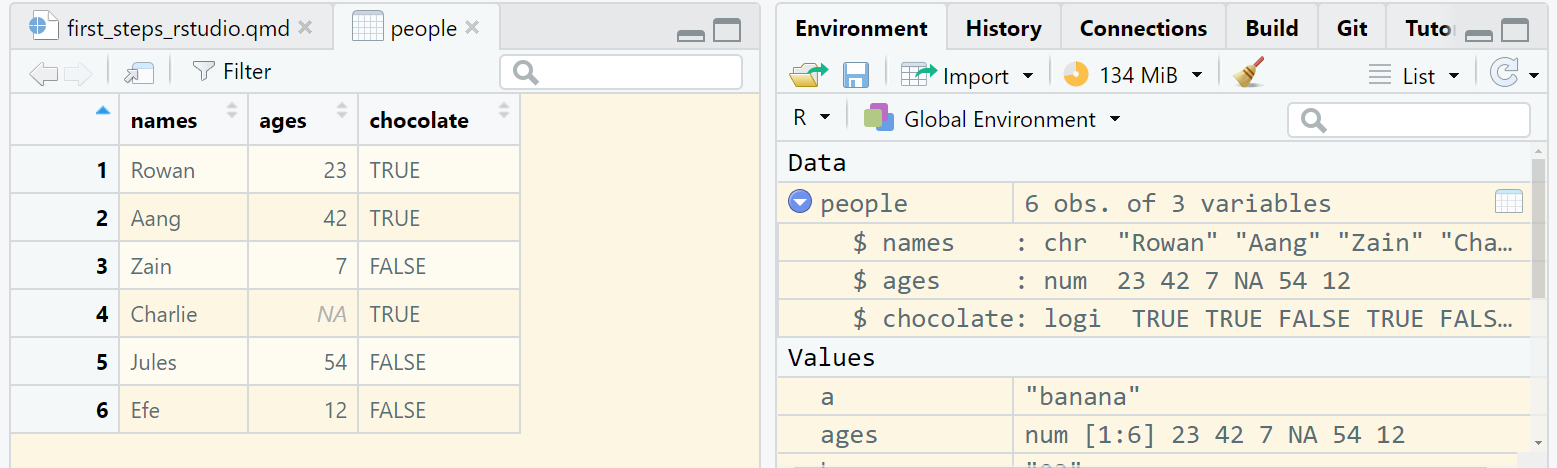
\includegraphics[width=8.33333in,height=\textheight]{images/view-dataframe.png}

}

\caption{\label{fig-view-dataframe}To open a spreadsheet-like view of
the dataframe click its name in the Global Environment}

\end{figure}

\hypertarget{tibbles}{%
\subsection{Tibbles}\label{tibbles}}

\hypertarget{summary}{%
\section{Summary}\label{summary}}

\hypertarget{workflow-in-rstudio}{%
\chapter{Workflow in RStudio}\label{workflow-in-rstudio}}

\begin{tcolorbox}[enhanced jigsaw, opacitybacktitle=0.6, toprule=.15mm, arc=.35mm, colback=white, colframe=quarto-callout-important-color-frame, opacityback=0, titlerule=0mm, colbacktitle=quarto-callout-important-color!10!white, leftrule=.75mm, breakable, bottomtitle=1mm, toptitle=1mm, title=\textcolor{quarto-callout-important-color}{\faExclamation}\hspace{0.5em}{Important}, rightrule=.15mm, bottomrule=.15mm, coltitle=black, left=2mm]

You are reading a work in progress. This page is a dumping ground for
ideas and not really readable. :::

\end{tcolorbox}

\hypertarget{understanding-the-pipe}{%
\section{\texorpdfstring{Understanding the pipe
\texttt{\textbar{}\textgreater{}}}{Understanding the pipe \textbar\textgreater{}}}\label{understanding-the-pipe}}

The pipe operator improves code readability by:

\begin{itemize}
\tightlist
\item
  structuring sequences of data operations left-to-right and top to
  bottom rather than from inside and out),
\item
  minimizing the need for intermediates,
\item
  making it easy to add steps anywhere in the sequence of operations.
\end{itemize}

For example, suppose we want to apply a log-square root transformation
which is sometimes applied to make a flat distribution more normal.
There are two approaches we could use without the pipe: nesting the
functions and creating an intermediate. We will consider both of these.
First, let us generate a few numbers of work with:

\begin{Shaded}
\begin{Highlighting}[]
\CommentTok{\# generate some numbers}
\CommentTok{\# this will give me ten random numbers between 1 and 100}
\NormalTok{nums }\OtherTok{\textless{}{-}} \FunctionTok{sample}\NormalTok{(}\DecValTok{1}\SpecialCharTok{:}\DecValTok{100}\NormalTok{, }\AttributeTok{size =} \DecValTok{10}\NormalTok{)}
\end{Highlighting}
\end{Shaded}

To apply the transformation we can nest the functions so the output put
of \texttt{sqrt(nums)} becomes the input of \texttt{log()}:

\begin{Shaded}
\begin{Highlighting}[]
\CommentTok{\# apply a log{-}square root transformation}
\NormalTok{tnums }\OtherTok{\textless{}{-}} \FunctionTok{log}\NormalTok{(}\FunctionTok{sqrt}\NormalTok{(nums))}
\NormalTok{tnums}
\end{Highlighting}
\end{Shaded}

\begin{verbatim}
 [1] 2.244318 2.124248 2.145230 2.249905 2.209420 1.647918 2.191013 2.102346
 [9] 1.818793 1.903331
\end{verbatim}

The first function to be applied is innermost. When we are using just
two functions, the level of nesting does not cause too much difficulty
in reading the code. However, you can image this gets more unreadable as
the number of functions applied increases. It also makes it harder to
debug and find out where an error might be. One solution is to create
intermediate variables so the commands a given in order:

\begin{Shaded}
\begin{Highlighting}[]
\CommentTok{\# apply a log{-}square root transformation}
\NormalTok{sqrtnums }\OtherTok{\textless{}{-}} \FunctionTok{sqrt}\NormalTok{(nums)}
\NormalTok{tnums }\OtherTok{\textless{}{-}} \FunctionTok{log}\NormalTok{(sqrtnums)}
\end{Highlighting}
\end{Shaded}

Using intermediates make your code easier to follow at first but
clutters up your environment and code with variables you don't care
about. You also start of run out names!

The pipe is a more elegant and readable solution. It allows you to send
the output of one operation as input to the next function. The pipe has
long been used by Unix operating systems (where the pipe operator is
\texttt{\textbar{}}). The R pipe operator is
\texttt{\textbar{}\textgreater{}}, a short cut for which is
Ctrl+Shift+M.

Using the pipe, we can apply out transformation with:

\begin{Shaded}
\begin{Highlighting}[]
\NormalTok{tnums }\OtherTok{\textless{}{-}}\NormalTok{ nums }\SpecialCharTok{|\textgreater{}} 
  \FunctionTok{sqrt}\NormalTok{() }\SpecialCharTok{|\textgreater{}} 
  \FunctionTok{log}\NormalTok{()}
\end{Highlighting}
\end{Shaded}

The command are in the order applied, there are no intermediates and the
code is easier to debug and to build-up step-by-step..

Note that \texttt{\textbar{}\textgreater{}} is the pipe that comes with
base R which was only added in the last couple of years. Before it
existed, \texttt{**tidyverse**} had a pipe operator provided by the
\texttt{*magrittr**} package. The magrittr pipe is
\texttt{\%\textgreater{}\%}. In your googling, you may well see code
written using the \texttt{\%\textgreater{}\%}. In most cases, the pipes
are interchangeable.

\hypertarget{rstudio-projects}{%
\section{RStudio Projects}\label{rstudio-projects}}

\begin{itemize}
\tightlist
\item
  \texttt{.RProj} indicates a folder is an RStudio Project
\end{itemize}

\hypertarget{folder-arrangement}{%
\section{folder arrangement}\label{folder-arrangement}}

\hypertarget{consistency}{%
\section{consistency}\label{consistency}}

\hypertarget{commenting}{%
\section{commenting}\label{commenting}}

\hypertarget{using-the-help}{%
\section{using the help}\label{using-the-help}}

\hypertarget{working-with-data-in-rstudio}{%
\chapter{Working with data in
RStudio}\label{working-with-data-in-rstudio}}

:::: status ::: callout-important You are reading a work in progress.
This page is a dumping ground for ideas and not really readable. :::

\begin{itemize}
\tightlist
\item
  importing data, types of file, different methds
\item
  summarising data, one two,
\item
  More plots
\item
  saving plots
\item
  tidying data
\end{itemize}

\hypertarget{getting-data-in-to-r}{%
\subsection{Getting data in to R}\label{getting-data-in-to-r}}

read\_table

\hypertarget{summarising-data}{%
\section{Summarising data}\label{summarising-data}}

concepts: mean, median, mode, standard deviation, sample distribution of
the mean, standard error

the role of data types in the type of summary

\hypertarget{summarising-and-plotting-a-single-variable}{%
\section{Summarising and plotting a single
variable}\label{summarising-and-plotting-a-single-variable}}

normal distribution, mean, sd, se, n, histogram categories mode, counts,
barchart,

using the help Your first plot! importing data, types of file, different
methds summarising data, one two, More plots saving plots tidying data

\bookmarksetup{startatroot}

\hypertarget{summary-1}{%
\chapter{Summary}\label{summary-1}}

\begin{tcolorbox}[enhanced jigsaw, opacitybacktitle=0.6, toprule=.15mm, arc=.35mm, colback=white, colframe=quarto-callout-important-color-frame, opacityback=0, titlerule=0mm, colbacktitle=quarto-callout-important-color!10!white, leftrule=.75mm, breakable, bottomtitle=1mm, toptitle=1mm, title=\textcolor{quarto-callout-important-color}{\faExclamation}\hspace{0.5em}{Important}, rightrule=.15mm, bottomrule=.15mm, coltitle=black, left=2mm]

You are reading a work in progress. This page is a dumping ground for
ideas and not really readable. :::

\end{tcolorbox}

\bookmarksetup{startatroot}

\hypertarget{keyboard-short-cuts-and-other-tips}{%
\chapter{Keyboard short cuts and other
tips}\label{keyboard-short-cuts-and-other-tips}}

:::: status ::: callout-important You are reading a work in progress.
This page is a dumping ground for ideas and not really readable. :::

\begin{longtable}[]{@{}
  >{\raggedright\arraybackslash}p{(\columnwidth - 6\tabcolsep) * \real{0.2917}}
  >{\raggedright\arraybackslash}p{(\columnwidth - 6\tabcolsep) * \real{0.2361}}
  >{\raggedright\arraybackslash}p{(\columnwidth - 6\tabcolsep) * \real{0.2361}}
  >{\raggedright\arraybackslash}p{(\columnwidth - 6\tabcolsep) * \real{0.2361}}@{}}
\toprule\noalign{}
\begin{minipage}[b]{\linewidth}\raggedright
Description
\end{minipage} & \begin{minipage}[b]{\linewidth}\raggedright
Item
\end{minipage} & \begin{minipage}[b]{\linewidth}\raggedright
Windows/ \& Linux
\end{minipage} & \begin{minipage}[b]{\linewidth}\raggedright
Mac
\end{minipage} \\
\midrule\noalign{}
\endhead
\bottomrule\noalign{}
\endlastfoot
All the Keyboard Shortcuts & & Alt+Shift+K & Option+Shift+K \\
Insert the Assignment operator & \texttt{\textless{}-} & Alt+- &
Option+- \\
Open a new script & & Ctrl+Shift+N & Shift+Command+N \\
Run current line/selection & & Ctrl-Enter & Command-Return \\
Comment out current line/selection & & Ctrl+Shift+C & Shift+Command+C \\
Open help on current function & & F1 & F1 \\
Insert the pipe operator & \texttt{\textbar{}\textgreater{}} &
Ctrl+Shift+M & Shift+Command+M \\
& & & \\
& & & \\
& & & \\
& & & \\
& & & \\
& & & \\
& & & \\
& & & \\
& & & \\
& & & \\
& & & \\
& & & \\
& & & \\
& & & \\
\end{longtable}

Alt+Shift+K

\bookmarksetup{startatroot}

\hypertarget{references}{%
\chapter*{References}\label{references}}
\addcontentsline{toc}{chapter}{References}

\markboth{References}{References}

\hypertarget{refs}{}
\begin{CSLReferences}{0}{0}
\end{CSLReferences}



\end{document}
